\documentclass[10pt]{article}
\usepackage{graphicx}
\usepackage{float}

\begin{document}
\title{Some Links are Hard, Some Links are Soft}
\author{Paul D. Camarata}
\date{28 August 2018}

\maketitle
\pagebreak

\section{Q1}
Results of ln -li file1.txt

\begin{figure}[H]
\centering
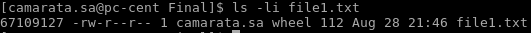
\includegraphics[scale=0.5]{./images/ss1.png}
\caption{ln -li file1.txt}
\label{ln -li file1.txt}
\end{figure}

What are the inode values of file1.txt and file2.txt?  Are they the same or different? Do the two files have the same or different contents?

Inode values are both 67109127. 

\begin{figure}[H]
\centering
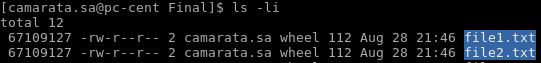
\includegraphics[scale=0.5]{./images/ss2.png}
\caption{ln -li}
\label{ln -li}
\end{figure}

file1.txt content is the same as file2.txt content.

\begin{figure}[H]
\centering
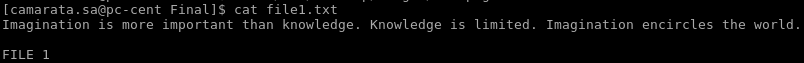
\includegraphics[scale=0.5]{./images/ss3.png}
\caption{cat file1.txt}
\label{cat file1.txt}
\end{figure}

\begin{figure}[H]
\centering
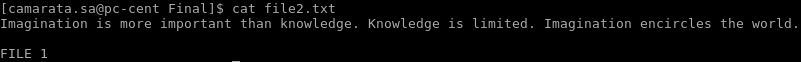
\includegraphics[scale=0.5]{./images/ss4.png}
\caption{cat file2.txt}
\label{cat file2.txt}
\end{figure}

\section{Q2}
Insert new content into file2.txt

\begin{figure}[H]
\centering
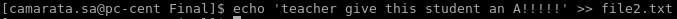
\includegraphics[scale=0.5]{./images/ss5.png}
\caption{echo >> file2.txt}
\label{echo >> file2.txt}
\end{figure}

The content of both files is still the same.

\begin{figure}[H]
\centering
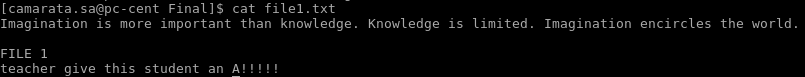
\includegraphics[scale=0.5]{./images/ss6.png}
\caption{cat file2.txt}
\label{cat file2.txt}
\end{figure}

It does not remove file2.txt as well

\begin{figure}[H]
\centering
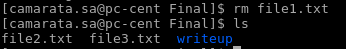
\includegraphics[scale=0.5]{./images/ss7.png}
\caption{rm file1.txt}
\label{rm file1.txt}
\end{figure}

Verbose removal of file2.txt.  It should be noted that rm by default is using the unlink() system call.

\begin{figure}[H]
\centering
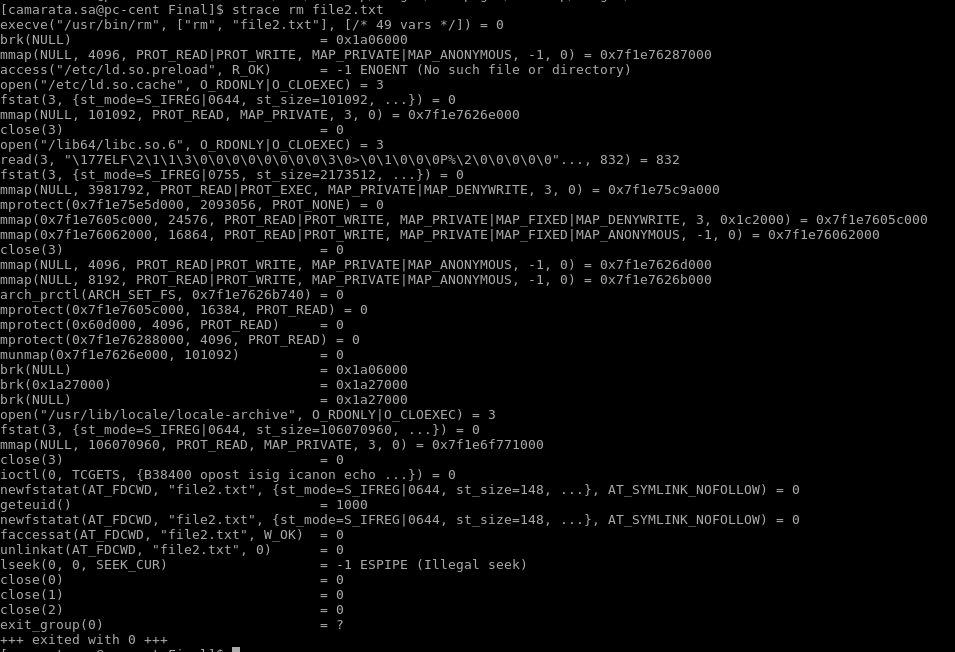
\includegraphics[scale=0.5]{./images/ss8.png}
\caption{strace rm file2.txt}
\label{strace rm file2.txt}
\end{figure}

\section{Q3}
Create a symblolic link of file3.txt to file4.txt

\begin{figure}[H]
\centering
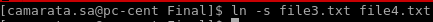
\includegraphics[scale=0.5]{./images/ss9.png}
\caption{ln -s file3.txt file4.txt}
\label{ln -s file3.txt file4.txt}
\end{figure}

inodes are different

\begin{figure}[H]
\centering
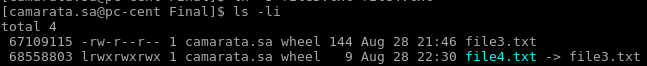
\includegraphics[scale=0.5]{./images/ss10.png}
\caption{ls -li}
\label{ls -li}
\end{figure}

Insert content into file4.txt

\begin{figure}[H]
\centering
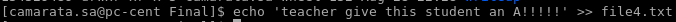
\includegraphics[scale=0.5]{./images/ss11.png}
\caption{echo >> file4.txt}
\label{echo >> file4.txt}
\end{figure}

View the content of file3.txt.  It is the same as file4.txt

\begin{figure}[H]
\centering
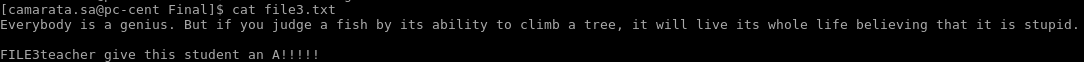
\includegraphics[scale=0.5]{./images/ss12.png}
\caption{cat file3.txt}
\label{cat file3.txt}
\end{figure}

remove file3.txt.  file4.txt is a broken link.

\begin{figure}[H]
\centering
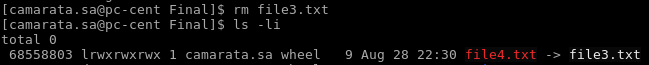
\includegraphics[scale=0.5]{./images/ss13.png}
\caption{rm file3.txt}
\label{rm file3.txt}
\end{figure}

Read from file4.txt

\begin{figure}[H]
\centering
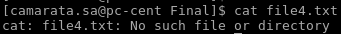
\includegraphics[scale=0.5]{./images/ss14.png}
\caption{cat file4.txt}
\label{cat file4.txt}
\end{figure}

You are unable to read from file4.txt.  The soft link still exists, but it is pointing to a non-existent hard link.  Because the file it is referencing is gone, it throws an error.

\pagebreak
\begin{thebibliography}{9}
\bibitem{OSConcepts}
Abraham Silberschatz, Peter Baer Galvin, Greg Gagne
\textit{Operating System Concepts}
John Wiley \& Sons Inc. 2018
\end{thebibliography}
\end{document}